\lecture{19}{2 maggio 2024}
\subsection{Polarizzatori}

Finora abbiamo considerato solo metalli con elettroni liberi di muoversi in ogni direzione. Esistono dispositivi in cui gli elettroni sono vincolati a muoversi in una sola direzione, rendendo il mezzo anisotropo. Nella figura si vede un esempio di come ciò può essere realizzato:
\begin{figure}[H]
	\centering
	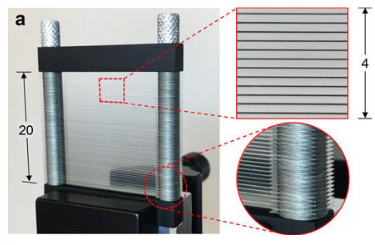
\includegraphics[width=0.4\textwidth]{screenshots/2024-05-02-09-16-09.png}
\end{figure}
Lungo i fili metallici si generano delle correnti (quindi effetto Joule e dispersione di energia), ma verticalmente gli elettroni non si possono muovere. Anche lunghe catene di idrocarburi possono realizzare lo stesso effetto (funzionano così le Polaroid e gli occhiali da sole).

Consideriamo un'onda elettromagnetica generica che si propaga lungo la direzione z con componenti casuali in x e y. Supponiamo di avere un polarizzatore nel piano xy, con le molecole orientate nella direzione y.
\begin{figure}[H]
	\centering
	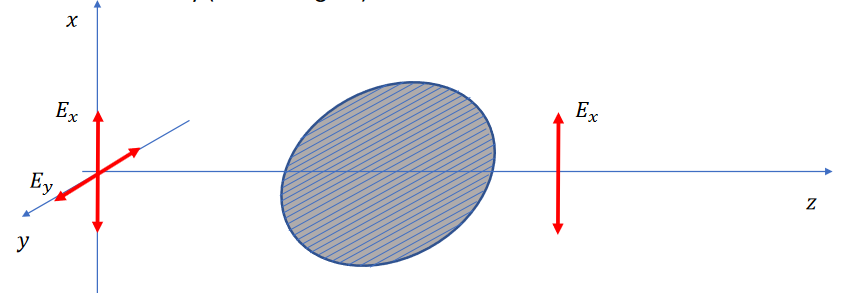
\includegraphics[width=0.6\textwidth]{screenshots/2024-05-02-09-19-57.png}
\end{figure}
Nel polarizzatore si realizza un forte assorbimento della componente y e un minimo di quella x. A valle del polarizzatore l'onda elettromagnetica è polarizzata linearmente lungo x.
\begin{note}
	Nei polarizzatori viene indicata sempre la direzione di trasmissione del campo elettrico, non la direzione dei fili! I fili sono perpendicolari alla direzione di trasmissione, perché assorbono il campo elettrico disperdendo la sua energia tramite effetto Joule.
\end{note}

L'intensità di un'onda diminuisce dopo il passaggio attraverso il polarizzatore. Inizialmente si ha
\begin{equation}
	I_0 = \left\langle \frac{E_x ^{2} + E_y ^{2} }{Z} \right\rangle = \left\langle \frac{2E_x ^{2} }{Z} \right\rangle 
\end{equation}
Se il polarizzatore è ideale, il campo elettrico su y viene annullato e il campo elettrico su x non varia, quindi l'intensità diventa
\begin{equation}
	I = \left\langle \frac{E_x ^{2} }{Z} \right\rangle = \frac{I_0}{2}
\end{equation}

Supponiamo invece di avere un'onda già polarizzata in direzione x che si propaga lungo la direzione z. Inoltre supponiamo di avere un polarizzatore nel piano xy, con un asse di trasmissione inclinato di un angolo \(\varphi _0\):
\begin{figure}[H]
	\centering
	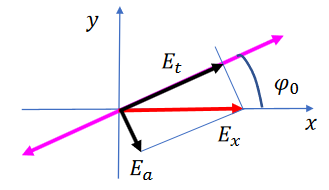
\includegraphics[width=0.4\textwidth]{screenshots/2024-05-02-09-28-03.png}
\end{figure}
\begin{formula}
	[Legge di Malus]
	Si ottiene così la legge di Malus:
	\begin{equation}
		I(\varphi _0) = \left\langle \frac{E_t ^{2} }{Z} \right\rangle = \left\langle \frac{E_x ^{2} \cos ^{2} (\varphi _0)}{Z} \right\rangle
		= I_0 \cos ^{2} (\varphi _0)
	\end{equation}
\end{formula}
\begin{note}
	La polarizzazione di questo tipo funziona con qualsiasi tipo di onda, non è specifica delle onde armoniche.
\end{note}

\paragraph{Mezzi anisotropi}
Vogliamo ora produrre polarizzazioni circolari ed ellittiche. Per ottenerle è necessario avere delle onde armoniche. Nella maggior parte dei mezzi dielettrici valgono \(\vec{P}= \varepsilon _0 \chi _e \vec{E}\) e \(\vec{D}= \varepsilon \vec{E}\) con \(\chi _e\) e \(\varepsilon \) sono quantità scalari. Nei mezzi anisotropi queste quantità sono tensori simmetrici di rango 2. La relazione resta lineare, ma il coefficiente di proporzionalità è un tensore. Ne consegue che la velocità di un'onda elettromagnetica dipende dal piano di oscillazione del campo elettrico (non dalla direzione di propagazione dell'onda!), perché l'indice di rifrazione sarà diverso nelle tre direzioni.
\begin{equation}
	n =
	\begin{pmatrix}
		\quotient{\varepsilon _x}{\varepsilon _0} & 0 & 0\\
		0 & \quotient{\varepsilon _y}{\varepsilon _0} & 0\\
		0 & 0 & \quotient{\varepsilon _z}{\varepsilon _0}\\   
	\end{pmatrix}
\end{equation}
Consideriamo un'onda armonica polarizzata incidente su una lamina di materiale anisotropo con \(n_x \neq n_y\), di spessore \(d\). Poniamo \(\vec{E}(z,t)=\quotient{E_0}{\sqrt{2} }  \cos (kz- \omega t)(\vec{\hat{i}} + \vec{\hat{j}})\) per \(z <0\). Se la lamina è tra 0 e d, la componente x ha velocità \(v_x \quotient{c}{n_x} \) e numero d'onda \(\omega \quotient{n_x}{c} \) e subisce uno sfasamento totale \(\Delta \Phi_x = k_x d = \frac{\omega d n_x}{c}\) (si ottiene imponendo la continuità in \(z=d\) fra la lamina e l'esterno). Analogamente la componente y ha una velocità \(v_y = \frac{c}{n_y}\) e subisce uno sfasamento \(\Delta \Phi _y = k_y d = \frac{\omega d n_y}{c}\). Quando \(\vert \Delta \Phi _y - \Delta \Phi _x \vert = \quotient{\pi }{2} \) si realizzano le condizioni di un'onda polarizzata circolarmente:
\begin{equation}
	\frac{\omega d n_x}{c} - \frac{\omega d n_y}{c} = \frac{\pi}{2} \rightsquigarrow d = \frac{\lambda }{4(n_x - n_y)}
\end{equation}
Per questo è detta "lamina a quarto d'onda".
Si ottengono così le seguenti descrizioni dell'onda:
\begin{figure}[H]
	\centering
	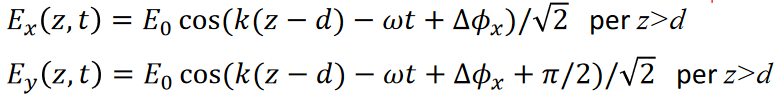
\includegraphics[width=0.4\textwidth]{screenshots/2024-05-02-09-49-04.png}
\end{figure}
Il campo elettrico si muove quindi "ad elica":
\begin{figure}[H]
	\centering
	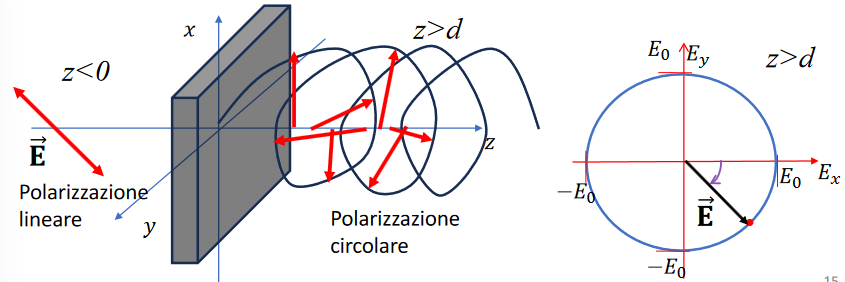
\includegraphics[width=0.5\textwidth]{screenshots/2024-05-02-09-50-10.png}
\end{figure}